\section{Ejercicio 2}

Distancia mínima y capacidad de corrección

Se tiene la distribución de pesos para el total de las palabras del código. La tabla se muestra en la siguiente figura:

\begin{figure}[h!]
    \centering
    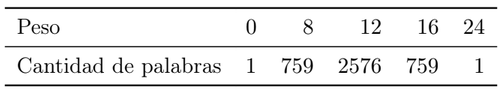
\includegraphics[scale=0.3]{img/code-weight-distribution.png}
    \caption{Tabla de distribución de pesos}
    \label{fig:code-weight-distribution}
\end{figure}

\subsection{Distancia mínima}

El código Golay es un código lineal, por lo que la distancia mínima es igual al menor peso no nulo de una palabra del código. Los pesos no nulos section 8, 12, 16 y 24. Por lo tanto se tiene que la distancia mínima es:

$$ \boxed{ d_{min} = 8 } $$

\subsection{Capacidad de correción}

La fórmula para el cálculo de la cantidad de errores que puede corregir el código es la siguiente:

$$ t = \frac{d_{min} - 1}{2} $$

Como se tiene que la distancia mínima $d_{min}= 8$, entonces se tiene:

$$ t = \frac{8-1}{2} = 3 $$

$$ \boxed{t = 3} $$

El código puede corregir hasta 3 errores por palabra recibida.

\subsection{Capacidad de detección}

Respecto a la capacidad de detección se tiene que el cálculo es el siguiente:

$$ d_{min} - 1 = 8 - 1 = 7 $$

$$ \boxed{ capacidad \, de \, detección = 7 } $$

El código Golay puede detectar hasta 7 errores.

\subsection{Detalles del código}

El algoritmo decodificador está diseñado para corregir patrones de hasta 3 errores. 
A raíz de esto puede ocurrir que se transmita una codeword $c_{1}$. La misma llega al decodificador con 5 errores.
Entonces se tiene que la palabra recibida es:

$$ r = c_{1} \xor e_{5}$$
